% Created 2023-11-07 Tue 04:39
% Intended LaTeX compiler: pdflatex
\documentclass[11pt]{article}
\usepackage[utf8]{inputenc}
\usepackage[T1]{fontenc}
\usepackage{graphicx}
\usepackage{longtable}
\usepackage{wrapfig}
\usepackage{rotating}
\usepackage[normalem]{ulem}
\usepackage{amsmath}
\usepackage{amssymb}
\usepackage{capt-of}
\usepackage{hyperref}
\usepackage{graphicx, tabularx}
\graphicspath{ {./images/} }
\author{Hankertrix}
\date{\today}
\title{Alkyl Halide Reactions Cheat Sheet}
\hypersetup{
 pdfauthor={Hankertrix},
 pdftitle={Alkyl Halide Reactions Cheat Sheet},
 pdfkeywords={},
 pdfsubject={},
 pdfcreator={Emacs 29.1 (Org mode 9.6.6)}, 
 pdflang={English}}
\begin{document}

\maketitle
\setcounter{tocdepth}{2}
\tableofcontents

\newpage

\section{Definitions}
\label{sec:orgf0a3068}

\subsection{Halogen}
\label{sec:org657e4b2}
Halogen just refers to group 7 elements in the periodic table.

\subsection{Nucleophiles}
\label{sec:org04f17ef}
A nucleophile is a chemical species that form bonds by donating an electron-pair. Nucleophiles are electron-pair donors. You can think of nucleophiles as electron haters, so they want to donate their electrons away.

\subsection{Organic halides (\(RX\))}
\label{sec:orgf3bd9c8}
Organic halides are organic compounds that contain one or more halogen atoms. The \(C - X\) bond is longer and hence weaker as you go down the periodic table. The \(C - X\) bond is polarised, and organic halides are often good starting materials in \textbf{nucleophilic substitution and elimination}.

\subsection{Polar protic solvents}
\label{sec:orgc3f1fa5}
Polar protic solvents are polar solvents that have at least 1 hydrogen that is connected directly to a particular electronegative atom, such as \(O-H, N-H\) and are capable of forming hydrogen bonds with the solute. Water is an example of a polar protic solvent.

\subsection{Polar aprotic solvents}
\label{sec:orgae8afa7}
Polar aprotic solvents are polar solvents that are unable to form hydrogen bonds with the solute. Examples include, acetone, chloroform, dichloromethane, ether, HMPA, DMSO, DMF and \(CH_3 CN\).

\subsection{Alpha carbon (\(\alpha\)-carbon)}
\label{sec:org58b5e75}
The alpha carbon is the \textbf{first} carbon atom that attaches to a functional group, like a halogen group.

\subsection{Beta carbon (\(\beta\)-carbon)}
\label{sec:orgbf60552}
The beta carbon is the second carbon atom that attaches to a function group, like a halogen group. The beta carbon atom is always the adjacent carbon atom to the alpha carbon atom.

\subsection{Zaitsev's rule}
\label{sec:orge90535b}
Zaitsev's rule states that the major product is the one with the \textbf{more substituted} double bonds.

\subsection{Hoffman's rule}
\label{sec:org18f445d}
Hoffman's rule states that the major product is the one with the \textbf{less substituted} double bonds.


\section{Nucleophilic substitution: \(S_N 2\) reactions}
\label{sec:orga88a93c}
\(S_N 2\) reactions are single step, and the \(S\) stands for substitution, \(N\) stands for nucleophilic, and 2 stands for bimolecular.
\[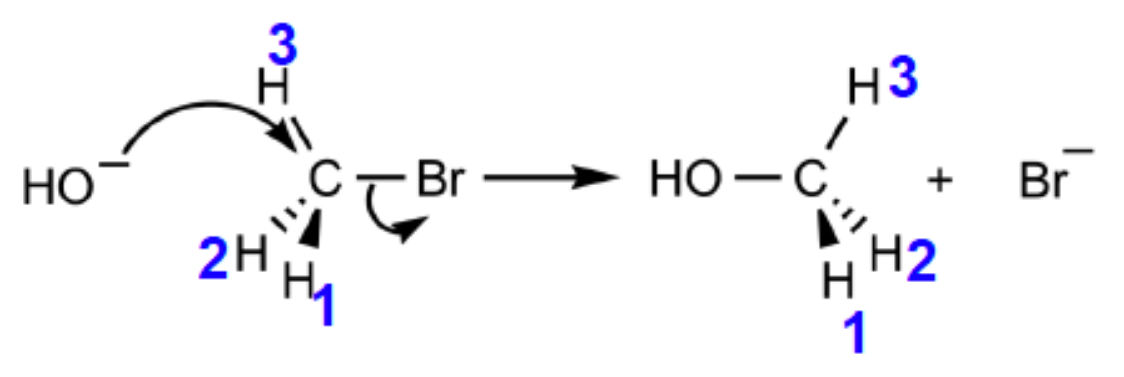
\includegraphics[width = \textwidth]{SN2}\]

\begin{itemize}
\item Configuration is \textbf{inverted} at the carbon where substitution occurs.
\item The formation of the new bond and the breaking of the old bond happens \textbf{simultaneously}.
\end{itemize}

The nucleophile attacks from the back side as the halogen simultaneously leaves from the front side. It is a one-step process.
\\[0pt]

There are 4 factors that affect \(S_N 2\) reactions:
\begin{enumerate}
\item Steric effects
\item Nucleophilic strength
\item Leaving group effects
\item Solvent effects
\end{enumerate}

\subsection{Steric effects}
\label{sec:org33b93a4}
The rate of \(S_N 2\) nucleophilic substitution reaction \textbf{increases} as the steric hindrance \textbf{decreases}. This is because it is much easier for the nucleophile to perform the backside attack when there are less bulky groups blocking the carbon atom.

\subsection{Nucleophilic strength}
\label{sec:org6e19a64}
\begin{itemize}
\item Nucleophilic strength decreases across the same row (left to right) in the periodic table.
\item Nucleophilic strength increases down the same group in the period table (in polar protic solvent).
\item Negative charge increases the nucleophilic strength.
\end{itemize}

\subsection{Leaving group effects}
\label{sec:org7b9107f}
\begin{itemize}
\item The more stable the negatively-charged leaving group, the better the leaving group.
\item Weak bases are usually good leaving groups as the negative charges are stabilised.
\item Bulky groups are often good leaving groups due to \textbf{resonance stabilisation}.
\item If a leaving group is very basic or small, it does not undergo the \(S_N 2\) reaction (e.g. alkyl fluoride, alcohols, ethers and amines do not undergo \(S_N 2\) reactions).
\item However, you can activate alcohols to make them better leaving groups.
\end{itemize}

\subsubsection{Conversion of alcohols to tosylate}
\label{sec:org0ff3687}
\[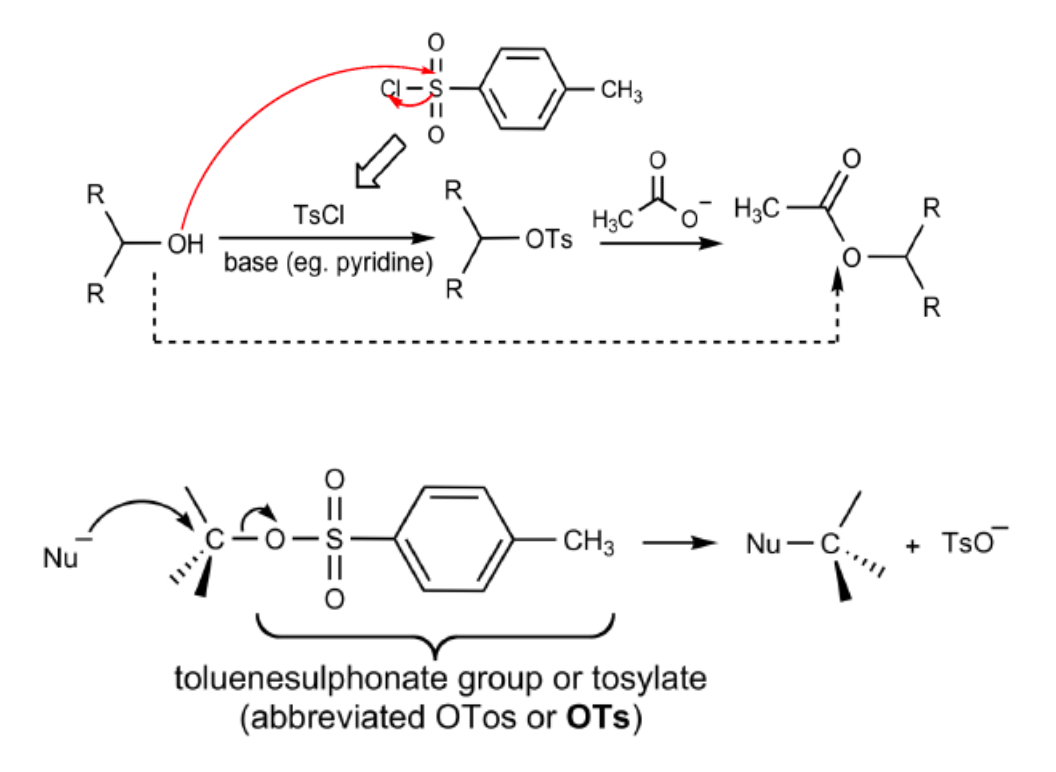
\includegraphics[width = \textwidth]{alcohol-to-tosylate}\]

\subsubsection{Conversion of alcohols to alkyl halides}
\label{sec:org19928fb}
\[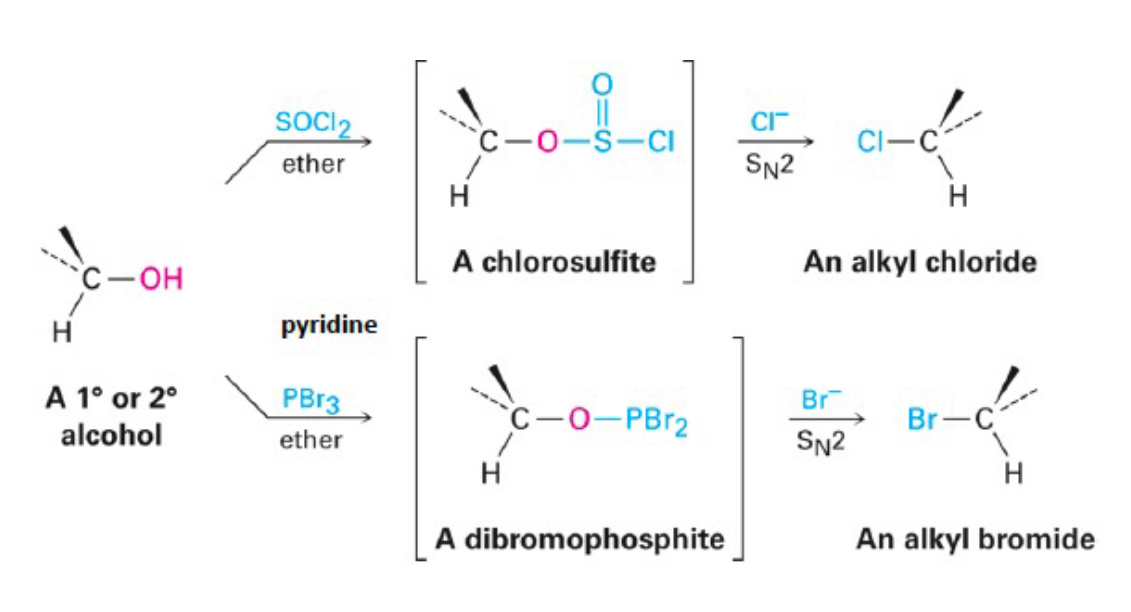
\includegraphics[width = \textwidth]{alcohol-to-alkyl-halide}\]

\subsection{Solvent effects}
\label{sec:org76ff159}
\begin{itemize}
\item Polar protic solvents form \(H\)-bond with the anion, which \textbf{lowers the reactivity} of the nucleophile.
\item Polar aprotic solvents \textbf{increase the reactivity of the nucleophiles} by stabilising the cation. They do not undergo hydrogen bonding with the anions.
\item Hence \textbf{polar aprotic solvents} are better for \(S_N 2\) reactions.
\end{itemize}

\section{Nucleophilic substitution: \(S_N 1\) reactions}
\label{sec:org30d54c3}
\(S_N 1\) reactions have two steps, and the \(S\) stands for substitution, \(N\) stands for nucleophilic, and 1 stands for unimolecular.
\[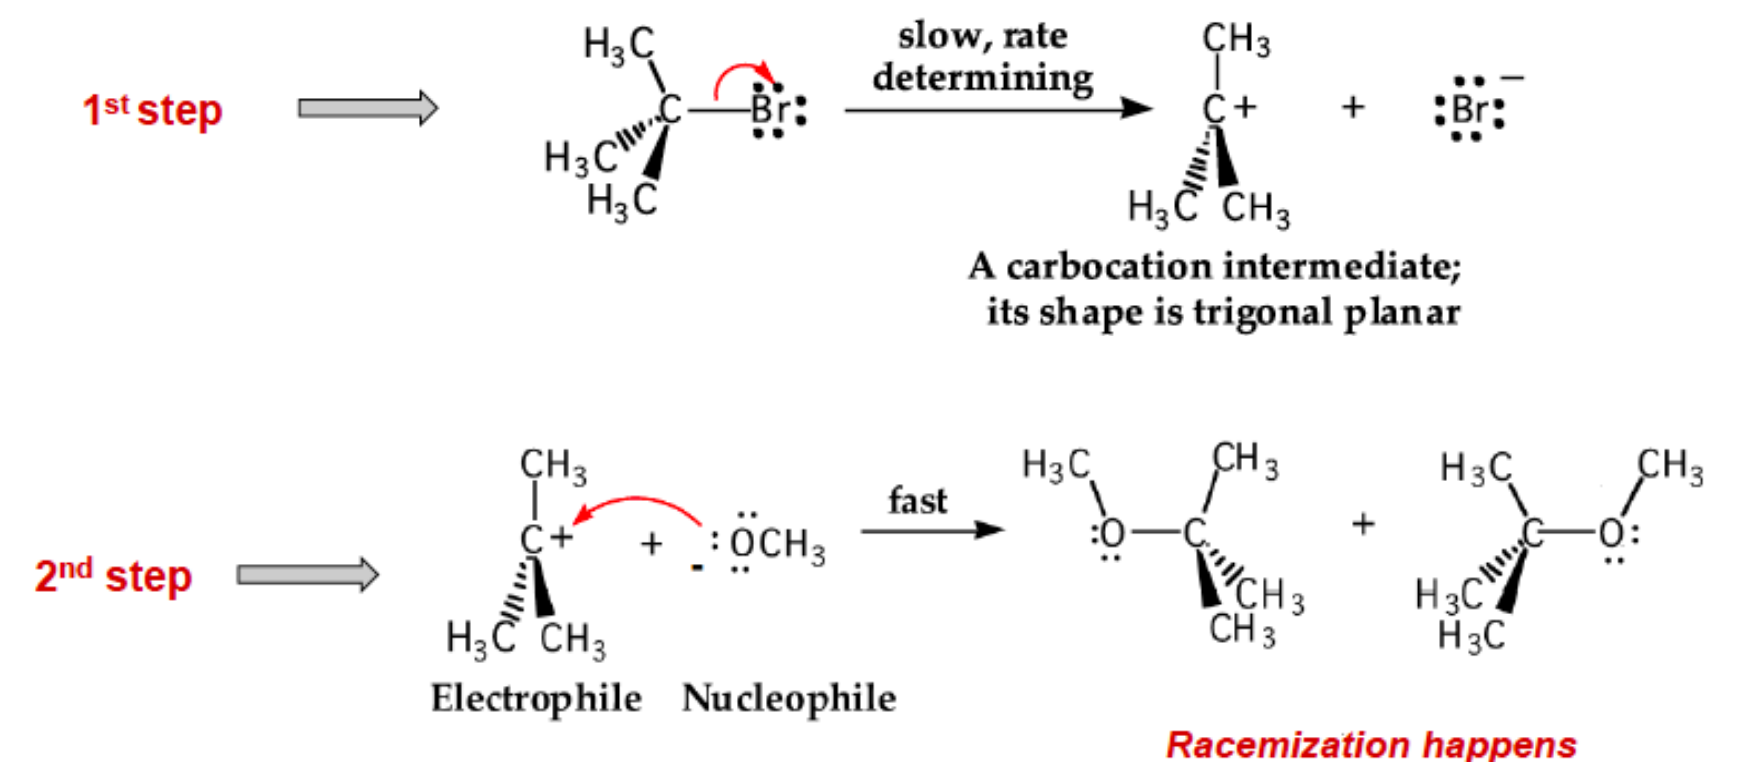
\includegraphics[width = \textwidth]{SN1}\]

\begin{itemize}
\item In the first step of the \(S_N 1\), the leaving group departs to generate a carbo-cation. The step is the slow step, or the rate-determining step.
\item The intermediate is \textbf{planar}, and hence the \textbf{chirality} is lost.
\item In the second step, the nucleophile attacks the carbo-cation. The product is a \textbf{racemic mixture} with 50\% of each enantiomer.
\end{itemize}

There are 3 factors that affect \(S_N 1\) reactions:
\begin{enumerate}
\item Substrate effects
\item Leaving group effects
\item Solvent effects
\end{enumerate}

\subsection{Substrate effects}
\label{sec:org258c0bc}
\begin{itemize}
\item Alkyl halides that can generate more \textbf{stable carbo-cations} are more reactive in the \(S_N 1\) pathway.
\item \textbf{Sterically bulky substituents} are preferred for \(S_N 1\) reactions, which is the opposite of \(S_N 2\) reactions.
\end{itemize}

\subsection{Leaving group effects}
\label{sec:org1ab597a}
\begin{itemize}
\item Good leaving groups facilitates \(S_N 1\) reactions, which is the same as \(S_N 2\) reactions.
\end{itemize}

\subsection{Solvent effects}
\label{sec:org1a29420}
The solvent influences the \textbf{transition state} and the \textbf{intermediate carbo-cation}.

\begin{itemize}
\item Polar solvents can stabilise the \(C^+\) in the transition state.
\item Polar protic solvents could also stabilise the leaving group.
\item Hence, polar protic solvents are ideal for \(S_N 1\) reactions.
\end{itemize}

\subsection{Nucleophilic strength}
\label{sec:org2a145ed}
Nucleophilic strength of the nucleophile is \textbf{not crucial} as the nucleophile is not involved in the rate determining step. Often, the nucleophile is the solvent itself.


\section{\(S_N 2\) versus \(S_N 1\)}
\label{sec:org953be1f}
\begin{tabular}{c|c|c}
& \(S_N 1\) & \(S_N 2\) \\
\hline
Electrophile & \(CH_3 X > 1^{\circ} > 2^{\circ}\) & \(3^{\circ} > 2^{\circ}\) \\
Nucleophile & Strong, unhindered base & Often the solvent \\
Rate & \(2^{nd}\) order & \(1^{st}\) order \\
Solvent & Polar protic & Polar aprotic \\
Leaving group & Weak base & Weak base \\
Stereochemistry & Inversion of configuration & Racemic mixture formed \\
\end{tabular}


\section{Elimination}
\label{sec:org66ba40d}
\begin{itemize}
\item Elimination reactions compete with nucleophilic substitution reactions in alkyl halides.
\item The nucleophile acts as the \textbf{base} by plucking the \(H\) atom on the \textbf{beta carbon atom}.
\item \textbf{Alkenes} are the result of elimination reactions.
\end{itemize}

There are 2 types of elimination reactions:
\begin{itemize}
\item E2 mechanism
\item E1 mechanism
\end{itemize}

\newpage

\subsection{E2 mechanism}
\label{sec:org8a26f83}
In the E2 mechanism, the breaking of the \(R-L\) and \(C-H\) bonds is simultaneous. The E2 mechanism is analogous to \(S_N 2\) reactions. The E stands for elimination and the 2 stands for bimolecular. The rate for the E2 mechanism is \(2^{nd}\) order.
\[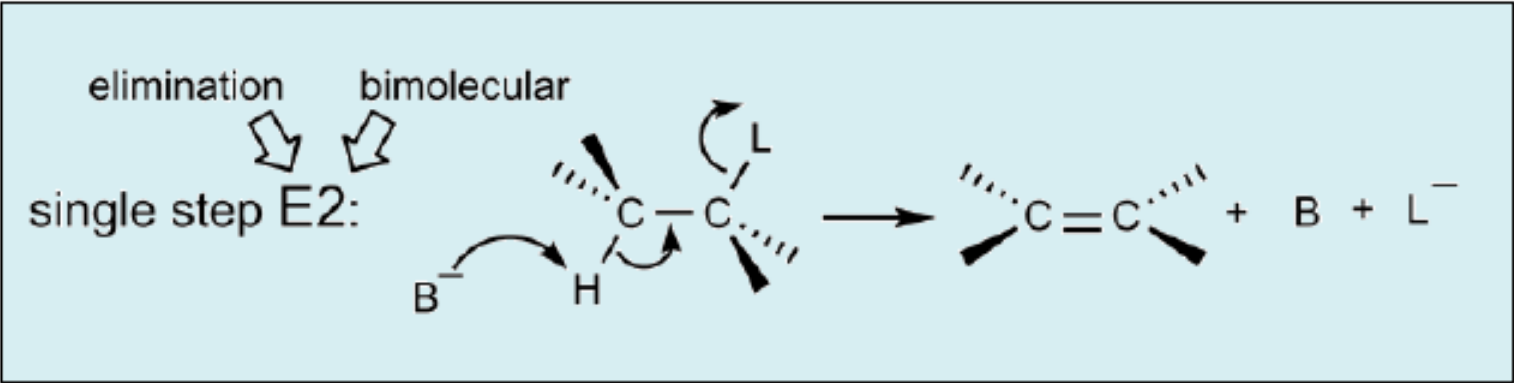
\includegraphics[width = \textwidth]{E2}\]

\begin{itemize}
\item The E2 mechanism is a single step reaction with the adduct "\(Nu-H-C-X\)" as the intermediate scaffold.
\item Nucleophiles attack the \(\beta-H\) bond to initialise the elimination.
\item E2 occurs in the presence of \textbf{strong bases} like \(OH^-\) or \(RO^-\).
\item Tertiary alkyl halides are good substrates for E2, which is unlike \(S_N 2\).
\end{itemize}

\subsubsection{Stereochemistry}
\label{sec:org4f06f25}
E2 occurs through an \textbf{anti-periplanar geometry} of the hydrogen atom bonded to the beta carbon and the halogen group. Basically, the hydrogen atom must be \(180^{\circ}\) away from the halogen, or the hydrogen atom must be on the opposite side of the halogen group.
\\[0pt]

This anti-periplanar requirement makes \textbf{E2 reactions stereospecific}. This means the stereochemistry of the product is controlled by the stereochemistry in the starting compound.

\subsubsection{Reaction in cyclohexyl halides}
\label{sec:orge8d07af}
\begin{itemize}
\item The hydrogen atom and the leaving group should align \textbf{trans-diaxial} to be anti-periplanar.
\item An \textbf{equatorial} leaving group \textbf{cannot} undergo elimination via the E2 mechanism.
\item So conformation matters in the E2 mechanism.
\end{itemize}

\newpage

\subsection{E1 mechanism}
\label{sec:orgb8ae868}
In the E1 mechanism, the breaking of the \(R-L\) bond generates a carbo-cation. The base then extracts the proton. The E1 mechanism is analogous to \(S_N 1\) reactions. The E stands for elimination and the 1 stands for unimolecular.
\[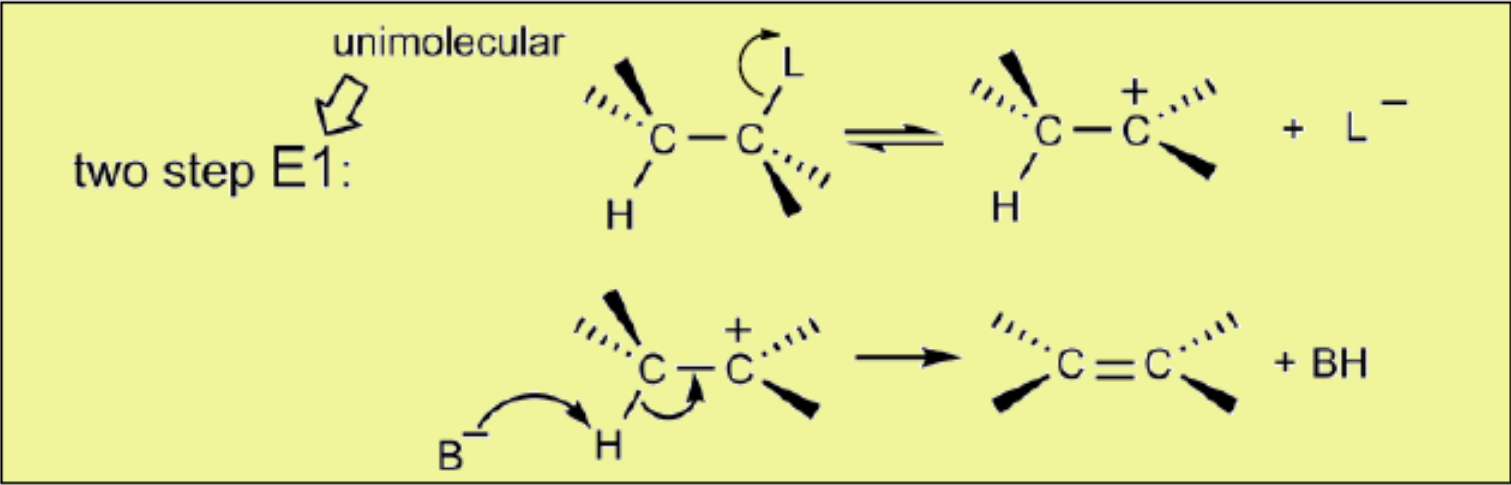
\includegraphics[width = \textwidth]{E1}\]

\begin{itemize}
\item E1 occurs with a \textbf{weak base} and under \textbf{acidic or neutral} conditions (similar to \(S_N 1\))
\item There is no anti-periplanar requirement for \(H\) and \(X\).
\item The E1 product often accompanies the product of a \(S_N 1\) reaction.
\item There are no geometric requirements for E1, which means E1 can take place in any conformation of the cyclohexane ring.
\end{itemize}

\subsection{Zaitsev's rule for elimination}
\label{sec:org009658d}
\begin{itemize}
\item Elimination often gives a mixture of products when there is more than \(\beta-H\).
\item The major product is the one with the \textbf{more substituted} double bonds.
\end{itemize}

There are exceptions to the Zaitsev's rule when the base is \textbf{bulky}. The base cannot extract the hydrogen atom on the more substituted carbon atom due to \textbf{steric hindrance}, and thus the major product is the one with \textbf{less substituted} double bonds. One example of such a base is tert-butoxide, \(C(CH_3)_3O^-\).


\section{E2 and E1 comparison}
\label{sec:org5f317d5}
\begin{tabularx}{\textwidth}{|c|>{\centering\arraybackslash}X|>{\centering\arraybackslash}X|}
\hline
& E2 & E1 \\
\hline
Rate law & Bimolecular (depends on the concentration of both the substrate and the base) & Unimolecular (depends on the concentration of the substrate) \\
\hline
Barrier & None & Formation of \newline carbo-cation \newline \(3^{\circ} > 2^{\circ} >> 1^{\circ}\) \\
\hline
Requires strong base? & Yes & No \\
\hline
Stereochemistry & Leaving group must be \textit{anti} to the hydrogen removed & No requirement \\
\hline
\end{tabularx}


\section{Summary of \(S_N\) and E}
\label{sec:org3645ab6}
\[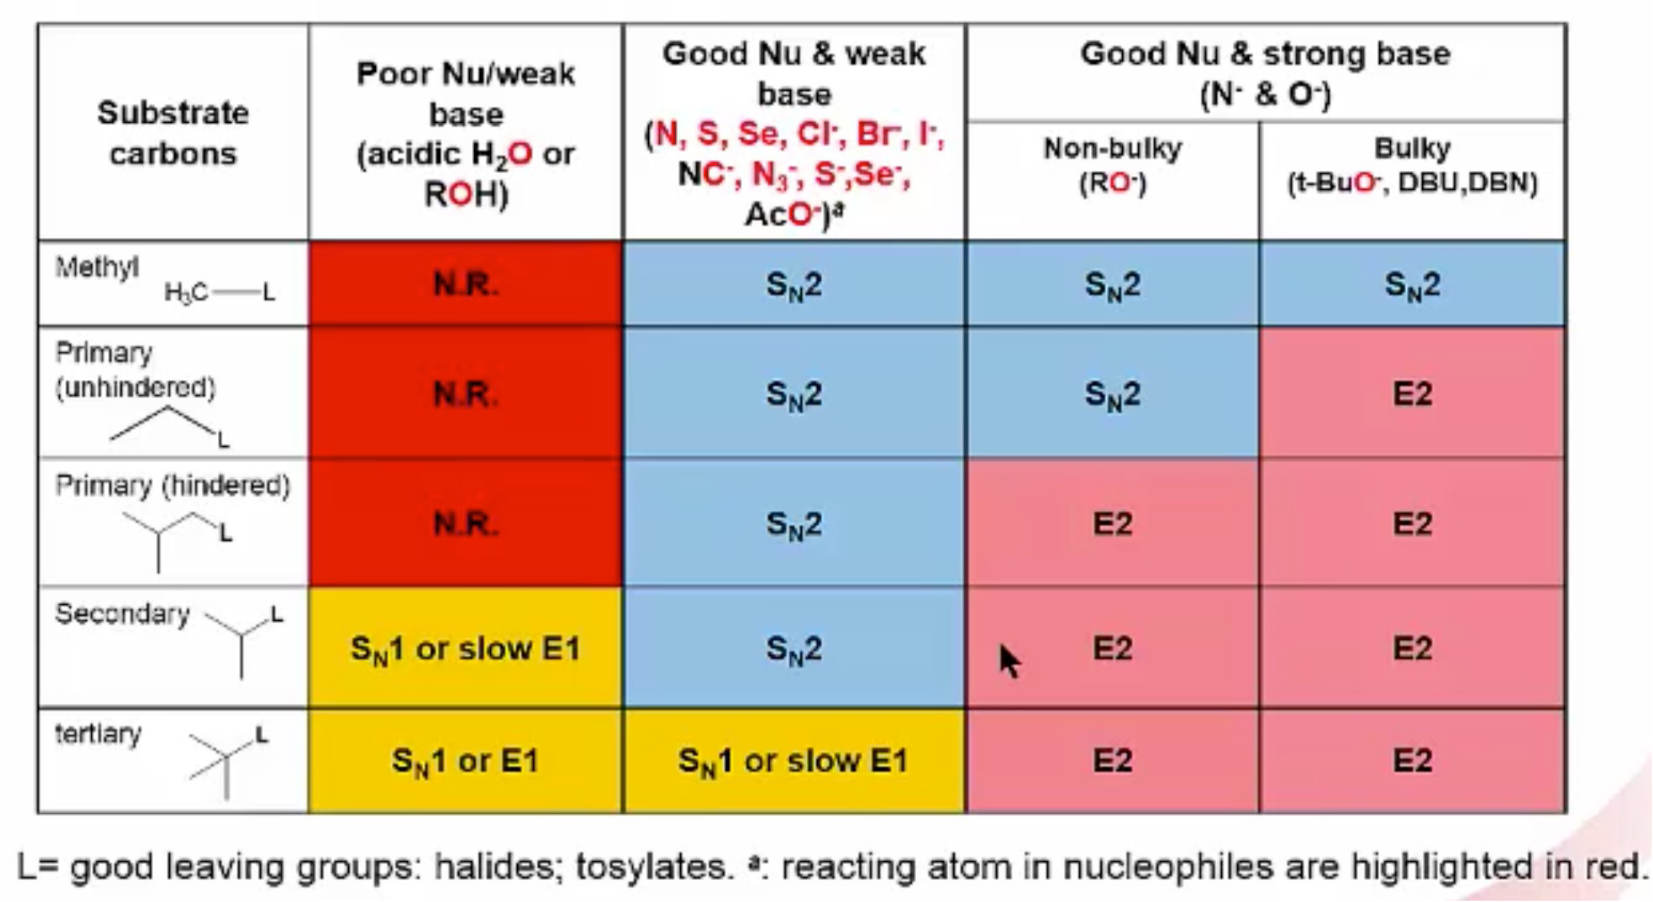
\includegraphics[width = \textwidth]{summary-of-sn-and-e}\]

\newpage

\section{Determining the mechanism of alkyl halide reactions}
\label{sec:orgf7f67ef}

\subsection{Step 1}
\label{sec:org52b670a}
Identify the type of carbon atom attached to the halogen atom.

\subsubsection{Primary halides (\(1^{\circ}\))}
\label{sec:orgda69896}
Primary halides can only undergo \(\boldsymbol{S_N 2}\) \textbf{and E2}.

\subsubsection{Secondary halides (\(2^{\circ}\))}
\label{sec:orgb4d22e6}
Secondary halides can undergo all alkyl halide reactions, so they can undergo \(\boldsymbol{S_N 1, S_N 2}\), \textbf{E1, and E2}.

\subsubsection{Tertiary halides (\(3^{\circ}\))}
\label{sec:orgf8ed5da}
Tertiary halides can only undergo \(\boldsymbol{S_N 1}\), \textbf{E1, and E2}.

\subsection{Step 2}
\label{sec:orgda6b3e2}
Identify the attacking group or the nucleophile.

\subsubsection{Weak nucleophile and weak base}
\label{sec:org9e21fb1}
Examples include acidic \(H_2 O\), \(ROH\), or any neutral molecule in general. The possible mechanisms for this situation are \(\boldsymbol{S_N 1}\) \textbf{and E1}.

\subsubsection{Weak nucleophile and strong base}
\label{sec:org55fe6c7}
Examples include bulky nucleophiles like t-Bu\(O^-\), DBU, and DBN. The only possible mechanism in this situation is \textbf{E2}.

\subsubsection{Strong nucleophile and weak base}
\label{sec:org8b8e831}
Examples include small nucleophiles like \(N, S, Se, Cl^-, Br^-, I^-, NC^-, N_3^-, S^-, Se^-, \text{ and } AcO^-\). The only mechanism for this situation is \(\boldsymbol{S_N 2}\).

\subsubsection{Strong nucleophile and strong base}
\label{sec:orgb8962e9}
Examples include non-bulky nucleophiles like \(RO^-\). The possible mechanisms for this situation are \(\boldsymbol{S_N 2}\) \textbf{and E2}.

\subsection{Step 3}
\label{sec:org42db5af}
Identify the solvent.

\subsubsection{Polar protic solvent}
\label{sec:orgb37b747}
Examples of polar protic solvents include water and alcohols. They favour \(\boldsymbol{S_N 1}\) \textbf{and E1} reactions, and disfavour \(S_N 2\) reactions.

\subsubsection{Polar aprotic solvent}
\label{sec:org28c5997}
Examples of polar \textbf{aprotic} solvents include acetone, ether, HMPA, and DMSO. Generally the solvents with names in capital letter are polar \textbf{aprotic} solvents. They favour \(\boldsymbol{S_N 2}\) reactions.

\subsubsection{Heat}
\label{sec:org1478242}
When there is heat, the mechanism is highly likely to be \textbf{E1}.
\end{document}